\section{Objetivos}

Em primeiro momento, o trabalho tem por objetivo fazer uma contextualização dos
métodos de cálculo e modelos utilizados, através de uma breve introdução
teórica. Contudo, o objetivo principal é construir um diagrama de equilíbrio
líquido-vapor (ELV) para um sistema binário contendo etano e propileno a 100 ºF.
Serão utilizadas diferentes equações de estado para prever as composições de ambas
as fases e os resultados serão comparados a dados experimentais obtidos da
literatura. Além disso, será feito um paralelo com o trabalho anterior, ou seja, 
se verificará a eficiência dos modelos das Leis de Raoult e Raoult Modificada
(UNIFAC(Do)) com aqueles utilizados no presente estudo. 



\section{Introdução Teórica}


\subsection{Equações de Estado} 

Conforme é apresentado por
\citeonline{SMITHJoeMauk;VANNESSHendrickC.;ABBOTT2007}, para a descrição do
comportamento de pressão, volume e temperatura (PVT) de um determinado fluido,
se faz necessário o uso de uma equação completa, a qual seja generalizada
suficientemente para ser aplicada a líquidos e gases.

As equações polinomiais, cúbicas no volume, são capazes de representar o
comportamento PVT de líquidos e vapores. A primeira equação de estado cúbica foi
proposta por J.D. van der Waals, no ano de 1873, e está apresentada na
\autoref{eq:vdw}

\begin{equation}\label{eq:vdw}
P = \frac{RT}{v - b} - \frac{a}{v^2}
\end{equation}
onde $P$ e $T$ são a pressão e temperatura absolutas, respectivamente; $R$ é a
constante universal dos gases; $v$ é o volume molar; $a$ e $b$ são constantes
positivas e, quando estas são nulas, obtem-se a equação dos gases ideais.

Equações de estado cúbicas no volume possuem três raizes distintas: as raízes
extremas (menor e maior) representam, quando se trata de um
equilíbrio líquido-vapor, os volumes molares das fases líquida e vapor,
respectivamente. Já a raiz intermediária não possui nenhum significado físico.

Com o passar do tempo, partindo-se a equação de van der Waals (vdW), diversas
outras equações de estado foram propostas. Dentre as mais conhecidas estão as
equações propostas por \citeonline{Redlich1949} (RK) e \citeonline{Peng1976}
(PR). De uma maneira genérica, pode-se expressar qualquer equação de estado a
partir da \autoref{eq:eqest}:

\begin{equation}\label{eq:eqest}
P = \frac{RT}{v - b} - \frac{a(T)}{(v + \epsilon b)(v + \sigma b)}
\end{equation}

 Os valores de $a$ e $b$ podem ser obtidos através das Equações \ref{eq:a} e
 \ref{eq:b}, onde $T_c$ e $P_c$ são a temperaturas e pressão críticas,
 respectivamente; $T_r$ e $P_r$ são a temperatura e pressão reduzidas,
 respectivamente, e estas são calculadas por meio das Equações \ref{eq:tr} e
 \ref{eq:pr}. O valor dos demais parâmetros, de acordo com cada equação de
 estado, está apresentado na \autoref{tab:eqest}

\begin{equation}\label{eq:a}
a = \displaystyle\frac{\Psi\alpha(T_r)R^2T_c^2}{P_c}
\end{equation}

\begin{equation}\label{eq:b}
b = \displaystyle\Omega\frac{RT_c}{P_c}
\end{equation}

\begin{equation}\label{eq:tr}
T_r = \displaystyle\frac{T}{T_c}
\end{equation}

\begin{equation}\label{eq:pr}
P_r = \displaystyle\frac{P}{P_c}
\end{equation}

\begin{table}[h]
\renewcommand{\arraystretch}{1.5}
\caption{Valores das constantes para diferentes equações de estado: vdW, RK e
PR}
\sisetup{table-format=3.9,round-mode=places,round-precision=5}
\footnotesize
\center
\begin{tabular}{SSSSSS[table-format=2.10,round-mode=places,round-precision=4]}
\toprule
   {Eq. de Estado} & {$\alpha T(r)$} & {$\sigma$} & {$\epsilon$} & {$
   \Omega $} & {$ \Psi $}\\
\midrule 
  {Ideal} & {0} & {0} & {0} & {0} & {0}\\
  {vdW} & {1} & {0} & {0} & {1/8} & {27/64}\\
  {RK} & {$\displaystyle\frac{1}{\sqrt{T_r}} $} & {1} & {0} & {0,08664} &
  {0,42748}\\
  %{SRK} & {$ {\alpha_{SRK}}^a $} & {1} & {0} & {0,08664} & {0,42748}\\
  {PR} & {$ {\alpha_{PR}}^* $} & {1 + $\sqrt{2}$} & {1 - $\sqrt{2}$} & {0,07780}
  & {0,45724}\\
    \midrule
 %\multicolumn{6}{l}
 %{$ ^a \alpha_{SRK} = [1+(0,48+1,547w-0,176w^2)(1-\sqrt{T_r})]^2$}\\
\multicolumn{6}{l}{$ ^* \alpha_{PR} = [1 +
 (0,37464+1,54226w-0,26992w^2)(1-\sqrt{T_r})]^2$}\\
\bottomrule
\multicolumn{6}{l}{Fonte: adaptado de
\citeonline{SMITHJoeMauk;VANNESSHendrickC.;ABBOTT2007}}
\end{tabular}
\label{tab:eqest}
\end{table}



\subsection{Equação de Redlich-Kwong (RK)}

A equação proposta por \citeonline{Redlich1949} está apresentada na
\autoref{eq:rkeq}.

\begin{equation}\label{eq:rkeq}
P = \frac{RT}{v - b} - \frac{a}{T^{1/2}v(v+b)}
\end{equation}

Os parâmetros $a$ e $b$ são escritos em termos da temperatura e pressão
críticas, utilizando a mesma metodologia que é aplicada à equação de
van der Waals. A equação de RK funciona bem para uma grande gama de condições,
porém se afasta significativamente dos valores medidos próximo ao ponto crítico
\cite{Koretsky2013}.



\subsection{Equação de Peng-Robinson (PR)}
  
 Diferentemente da equação proposta por \citeonline{Redlich1949}, que usa duas
 constante críticas para a estimação dos parâmetros (temperatura e pressão
 críticas), a equação de \citeonline{Peng1976}, apresentada na
 \autoref{eq:PReq}, faz o uso de um terceiro parâmetro, denotado de fator
 acêntrico de Pitzer ($w$). Com esse novo parâmetro, espera-se que esse modelo
 seja melhor aplicado para diferentes classes de moléculas \cite{Koretsky2013}:
  
  
  
 \begin{equation}\label{eq:PReq}
P = \frac{RT}{v - b} - \frac{\alpha T(r)}{v(v+b)+b(v-b)}
\end{equation} 

O valor de $\alpha T(r)$ é descrito na \autoref{eq:alfa}:
 \begin{equation}\label{eq:alfa}
\alpha T(r) = [1 +
 (0,37464+1,54226w-0,26992w^2)(1-\sqrt{T_r})]^2
\end{equation} 

 
 O fator acêntrico de Pitzer caracateriza o quão ``não-esférica'' é a molécula,
 assim, pode ser atribuída para uma classe de substâncias com
 características semelhantes. A \autoref{eq:w} apresenta a definição desse fator
 acêntrico:
 
  \begin{equation}\label{eq:w}
w \equiv -1 - log_{10}\left [ P^{sat} \left ( T_r = 0,7 \right )/P_c \right ]
\end{equation} 
onde $ P^{sat} \left ( T_r = 0,7 \right )$ é a pressão de saturação de dada
substância em uma termperatura reduzida igual a 0,70.



\section{Metodologia}

\subsection{Dados experimentais}
Os dados experimentais do equilíbrio utilizados foram retirados de \citeonline{McKay1951}. Trata-se de uma mistura binária contantendo dois
hidrocarbonetos: etano (1) e propileno (2) em uma temperatura de 100 ºF. Esses
valores coletados estão mostrados na \autoref{tab:dadosexp} .

\begin{table}[htb]
\renewcommand{\arraystretch}{1.3}
\caption{Dados experimentais do equilíbrio líquido-vapor da mistura
etano(1)/propeno(2) a 100 ºF.}
\sisetup{table-format=2.4,round-mode=places,round-precision=3}
\footnotesize
\center
\begin{tabular}{SSS[table-format=4.1,round-mode=places,round-precision=0]}
\toprule
   {$x_1$} & {$y_1$}& {$P$ (psi)} \\ 
\midrule 
  0,000 & 0,000 & 227 \\
  0,048 & 0,118 & 250 \\
  0,157 & 0,317 & 300 \\
  0,260 & 0,447 & 350 \\
  0,361 & 0,543 & 400 \\
  0,461 & 0,626 & 450 \\
  0,554 & 0,697 & 500 \\
  0,643 & 0,759 & 550 \\
  0,727 & 0,813 & 600 \\
  0,809 & 0,863 & 650 \\
  0,894 & 0,912 & 700 \\
  0,930 & 0,930 & 722 \\
\bottomrule
\multicolumn{2}{l}{Fonte: adaptado de \citeonline{McKay1951}}
\end{tabular}
\label{tab:dadosexp}
\end{table}
%\clearpage

\subsection{Método da igualdade de fugacidades ($\phi-\phi$)}

Os valores para a construção do diagrama de equilíbrio serão obtidos
através de cálculos de ponto de bolha, o qual fará uso de duas equações de
estados distintas: Peng-Robinson (PR) e Redlich-Kwong (RK). Para isso, se fará
necessário o uso do método de igualdade de fugacidade ($\phi-\phi$), conforme
mostra a \autoref{eq:fug}:

\begin{equation}\label{eq:fug}
\hat{f}_i^v = \hat{f}_i^l
\end{equation}
onde $\hat{f}_i^v$ e $\hat{f}_i^l$ são as fugacidades de cada componente, quando
em mistura, na fases vapor e líquida, respectivamente.

A fugacidade, por sua vez, pode ser expressa pelo produto entre a pressão do
sistema e a composição da fase ($x_i$ ou $y_i$), além de um coeficiente que
indica o desvio com relação à idealidade, chamdo de coeficiente de fugacidade
($\hat{\phi}_i$), conforme é mostrado na \autoref{eq:fug2}

\begin{equation}\label{eq:fug2}
Py_i\hat{\phi}_i^v = Px_i\hat{\phi}_i^l
\end{equation}

Para a condição de equilíbrio ser satisfeita, a pressão da fase líquida deve ser
a mesma da fase vapor. Logo, a \autoref{eq:fug2} pode ser reescrita como é
apresentado na \autoref{eq:fug3}.

\begin{equation}\label{eq:fug3}
y_i\hat{\phi}_i^v = x_i\hat{\phi}_i^l
\end{equation}

Para uma substância pura, os coeficientes de fugacidade da fase líquida
($\phi_i^l$) e da fase vapor ($\phi_i^v$) são iguais e possuem o mesmo valor de
coeficiente de fugacidade de saturação ($\phi_i^{sat}$), como mostra a
\autoref{eq:phi}.

\begin{equation}\label{eq:phi}
\phi_i^v = \phi_i^l = \phi_i^{sat}
\end{equation}



\subsection{Equações de Estado}
A determinação do valor do coeficiente de fugacidade, para ambas as fases, será
feita através de duas equações de estado distintas: Redlich-Kwong e
Peng-Robinson. Para os cálculos, utilizou-se o simulador de
processos $iiSE$. Os códigos de programação foram implementados em
liguagem $Java$ utilizando o ambiente do Eclipse Mars Release (4.5.0).



\section{Resultados} 

A \autoref{fig:pxy} apresenta os resulados obtidos utilizando o método de
igualdade de fugacidades ($\phi-\phi$). Nesse diagrama, estão mostrados os
valores experimentais e, também, aqueles calculuados fazendo-se o
uso das equações de Redlich-Kwong e Peng-Robinson.

É possível notar que a equação de estado de Peng-Robinson consegue prever, com
melhor confiabilidade, os valores das propriedades no equilíbrio. Percebe-se
que, além dessa equação (PR) estimar valores muito próximos daqueles ditos
reais, não há grandes desvios nos pontos iniciais (o que não ocorre quando
utiliza-se RK). A equação RK se mostra ruim na predição da região de propileno
como substância pura (pressão a qual $x_1$ é igual a zero).


\begin{figure}[htb]
\centering
{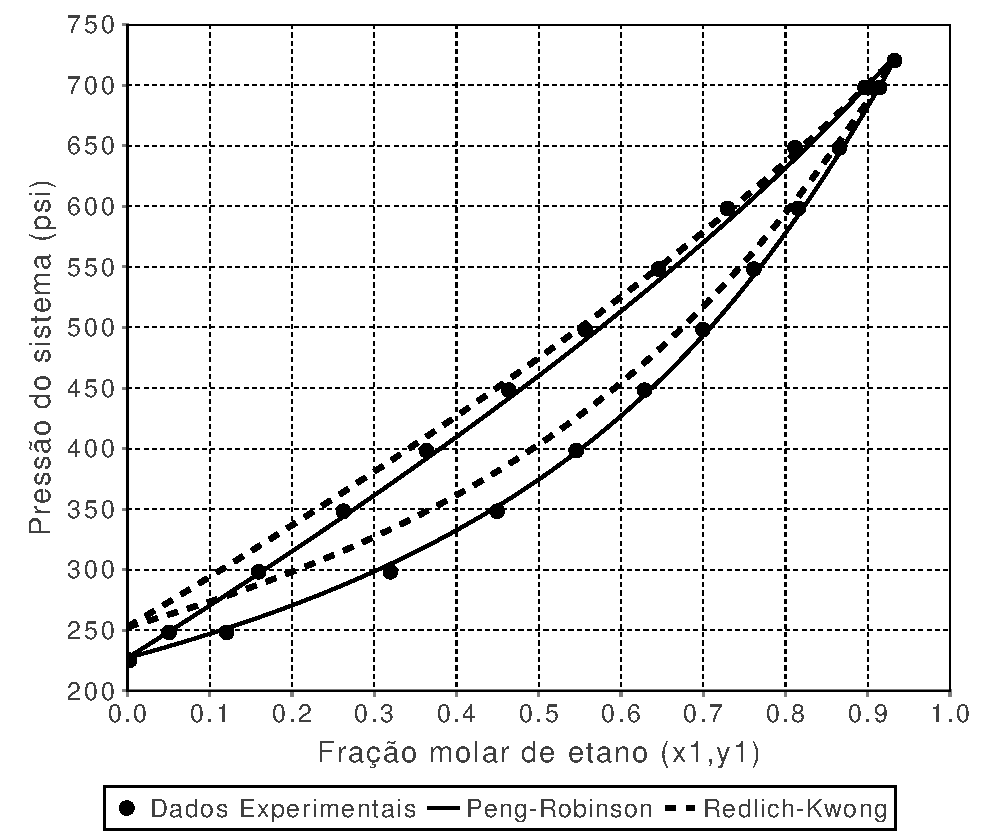
\includegraphics[width=0.8\textwidth]{img/trab2_pxy.pdf}} 
\caption{Diagrama de equilíbrio $P-xy$ da mistura de de etano (1) e
propileno (2) calculados com as equações de estado PR e RK}
\label{fig:pxy}
\end{figure} 

Ao analisar a \autoref{fig:xy}, que mostra um diagrama $y_1$ $versus$  $x_1$,
nota-se que a equação de estado de Peng-Robinson aproxima melhor os valores
calculados daqueles experimentais, quando comparado com a equação
Redlich-Kwong, a qual apresenta valores abaixo dos reais. Todavia, observa-se,
também, que a regra de mistura para ambas as equações são boas, pois os
comportamentos estão próximos aos valores experimentais.

\clearpage

\begin{figure}[htb]
\centering
{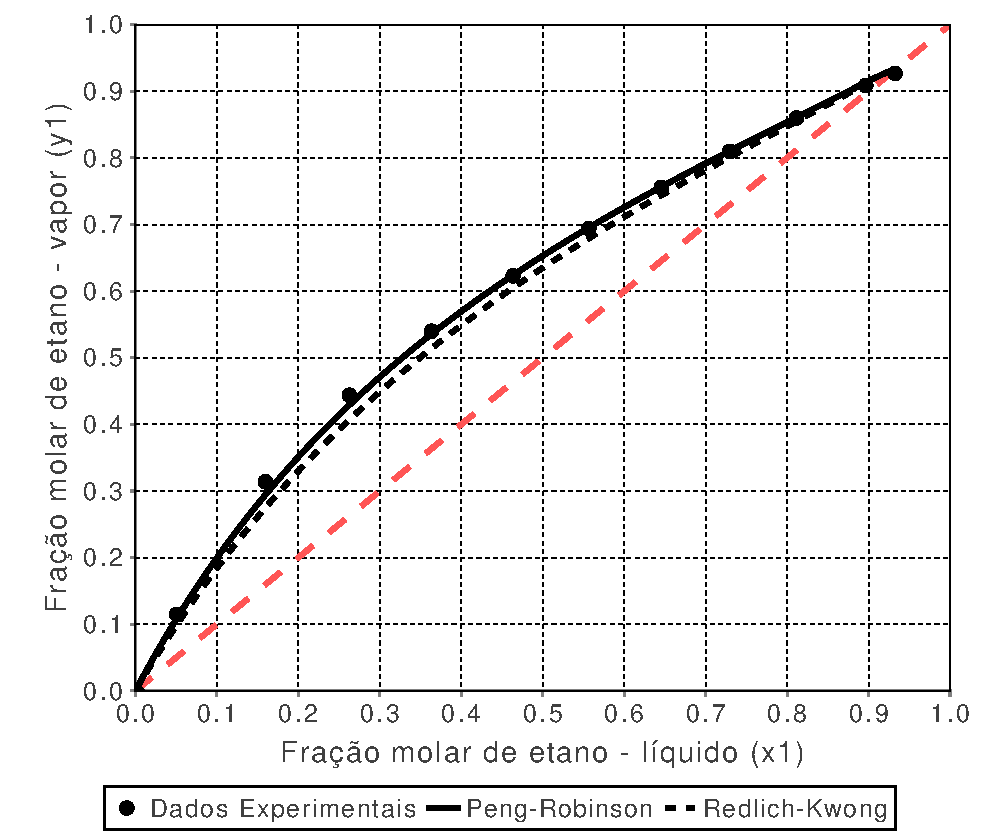
\includegraphics[width=0.8\textwidth]{img/trab2_xy.pdf}}
\caption{Diagrama de equilíbrio $x-y$ da mistura de de etano (1) e
propileno (2) calculados com as equações de estado PR e RK} 
\label{fig:xy}
\end{figure} 


Uma última comparação está apresentada na \autoref{fig:compare}, que ilustra
a diferença entre a utilização do método da igualdade de fugacidades
($\phi-\phi$) - o qual considera ambas as fases como sendo não ideais; Lei de
Raoult Modificada (com modelo UNIFAC modificação Dortmund \cite{Jakob2006} para
cálculo do coeficiente de atividade $\gamma_i$) - o qual considera a fase líquida não ideal
e a fase vapor sendo um gás ideal; e, por fim a Lei de Raoult - a qual faz 
consideração de ambas as fases ideais.

Ao analisar-se os gráficos apresentados na \autoref{fig:compare}, pode-se perceber
claramente que os dois modelos da Lei de Raoult apresentam
valores com erros maiores, comparando-se com aqueles calculados pelo método
$\phi-\phi$ e, também, não conseguem prever as propriedades no ponto crítico.
Como os dois modelos de Raoult consideram a fase vapor como sendo um gás ideal
e, como o sistema encontra-se em alta pressão, esse tipo de desvio já era esperado, visto
que convem-se utilizar equações de estado para esses casos.

\clearpage

\begin{figure}[htb] 
\centering
\subfloat[$P-xy$: PR e RK.]
{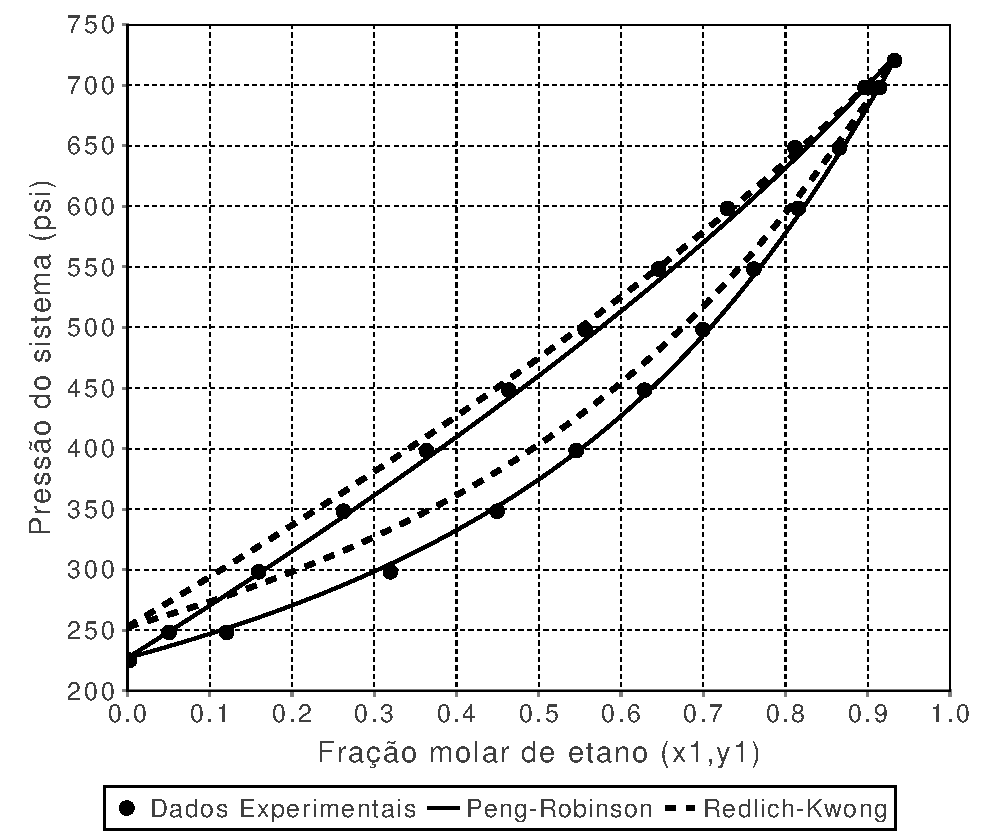
\includegraphics[width=0.5\textwidth]{img/trab2_pxy.pdf}}
\subfloat[$P-xy$: Leis de Raoult e Raoult Mod. (UNIFAC(Do)).]
{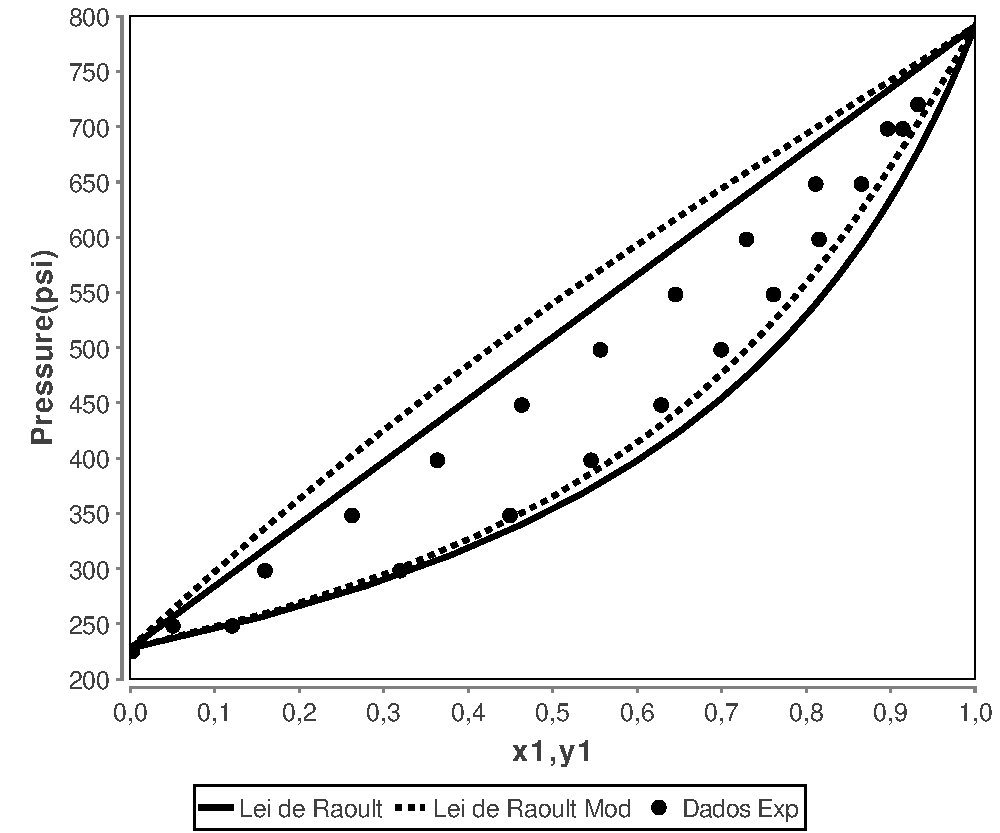
\includegraphics[width=0.5\textwidth]{img/VLE-Ethane(1)Propylene(2)-x1y1&Pressure-Raoult-RaoultMod.pdf}}\\
\subfloat[$x-y$: PR e RK.]
{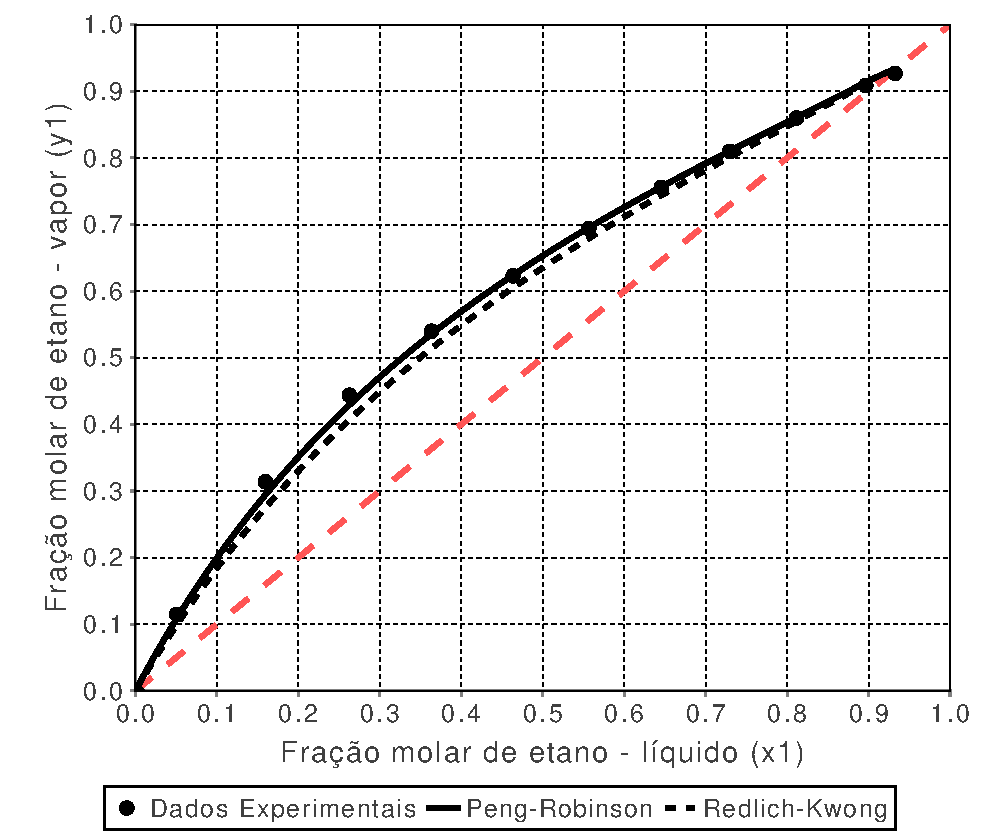
\includegraphics[width=0.5\textwidth]{img/trab2_xy.pdf}}
\subfloat[$x-y$: Leis de Raoult e Raoult Mod. (UNIFAC(Do)).]
{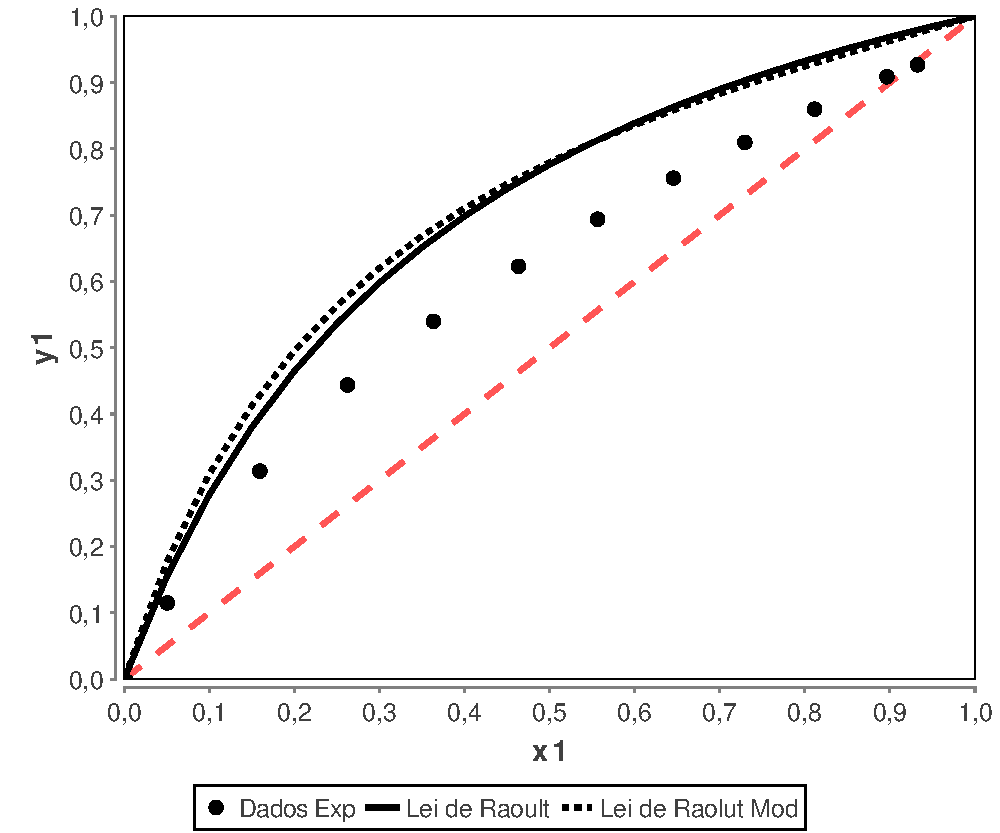
\includegraphics[width=0.5\textwidth]{img/VLE-Ethane(1)Propylene(2)-x1&y1-Raoult-RaoultMod.pdf}}
\caption{Comparação entre os métodos utilizados para a construção do diagrama 
de equilíbrio líquido-vapor da mistura etano(1) / propileno (2) a 100 ºF}
\label{fig:compare} 
\end{figure}



\section{Conclusões} 

O presente trabalho visou a construção de diagramas de equilíbrio líquido -
vapor de uma mistura binária contendo etano e propileno através do cálculo do ponto de bolha. Para isso, foi usado o método da igualdade de fugacidades (considerando
ambas as fases como não ideais) e testou-se duas equações de estado distintas
para o cálculo dos coeficientes de fugacidade.

Também foi feita uma comparação dos resultados obtidos com aqueles estimados na
atividade anterior (Atividade 1), a qual usou-se as Leis de Raoult e
Raoult Modificada com o modelo de UNIFAC(Do) para o cálculo do coeficiente de
ativiadade.

Com os resultados apresentados, foi possível concluir que, para o sistema em
questão, as equações de estado conseguiram prever muito melhor as propriedades
de equilíbrio, além de prever bem as propriedades próximas ao ponto 
crítico.
Como o sistema encontra-se em altra pressão, não é viável utilizar-se modelos da Lei de Raoult, pois esse
tipo de equação considera o vapor como uma gás ideal, o que torna a
estimação dos valores mal sucedida.

Quando comparou-se as duas equações de estados utilizadas no método $\phi-\phi$,
notou-se que Peng-Robinson preveu muito melhor os valores de pressão e
composição do que o modelo de Redlich-Kwong. A grande diferença está no fato de 
RK fazer a utilização de apenas duas constantes críticas para a estimação de
parâmetros ($T_c$ e $P_c$) e a equação de PR usar um terceiro parâmetro (fator acêntrico 
de Pitzer - $w$), fazendo com que tenha mais confiabilidade na prediaçãos de
dados de equilíbrio.

